\chapter{Super-resolution imaging}

\section{Objective}
\begin{itemize}
\item Super-resolution is an mage processing technique that
  increases the perceived quality by means of ``frabricaing''
  (possiblely \popup{unreal}{Invented.}) new visual information.
\item Even knowing this fact, it can help in medical imaging
  diagnosis.
\end{itemize}

\section{Nearest-neighbor interpolation}
\begin{itemize}
\item For a discrete image $f: \mathbb{Z}^2 \to \mathbb{R}$, the interpolation at a point 
$(x,y) \in \mathbb{R}^2$ is given by
\begin{equation}
\hat{f}(x,y) = f\!\left( \operatorname{round}(x), \operatorname{round}(y) \right),
\end{equation}
where $\operatorname{round}(x)$ returns the nearest integer value of $x$. 
\vspace{-2.5ex}
\begin{center}
  \href{https://www.mrecacademics.com/DepartmentStudyMaterials/20201220-Digital%20Image%20Processing%20Notes.pdf}{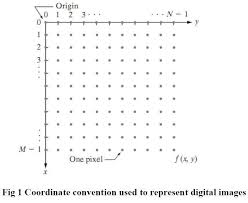
\includegraphics[width=6cm]{discrete_image}}
\end{center}
\item Simple, but can cause blocky artifacts.
\begin{center}
  \href{}{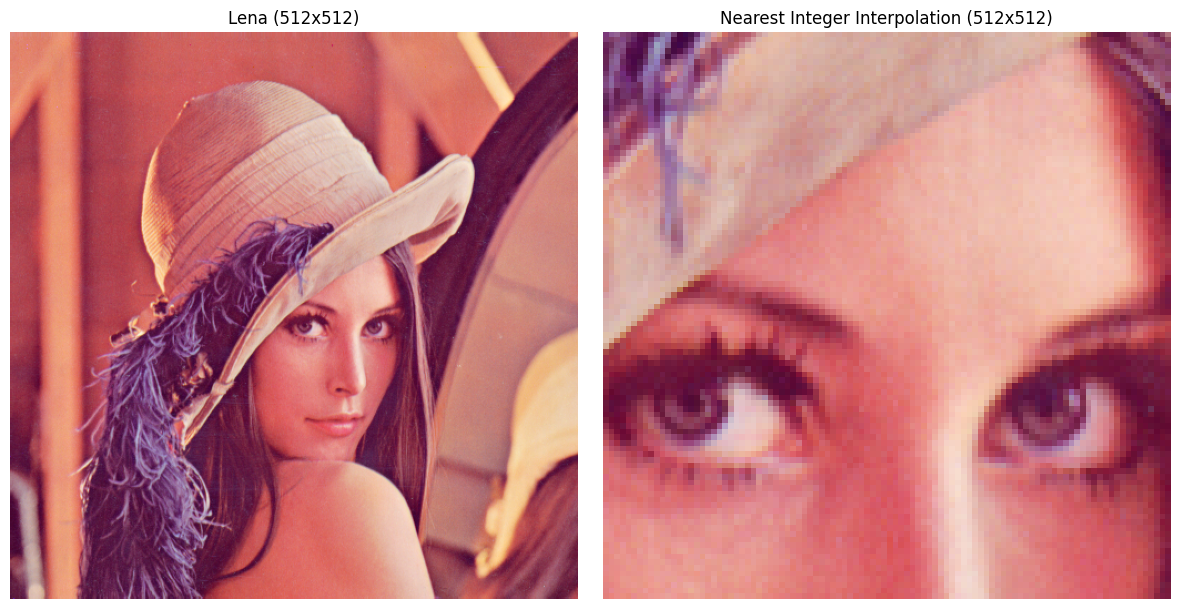
\includegraphics[width=12cm]{lena_nearest_integer}}
\end{center}
\end{itemize}

\section{Linear / bilinear / trilinear interpolation}

Smooth transitions, commonly used in CT/MRI resampling.

% ---------- Linear interpolation (1D) ----------
For a discrete signal $f: \mathbb{Z} \to \mathbb{R}$, the linear interpolation 
at a real position $x \in \mathbb{R}$ is given by
\[
\hat{f}(x) = (1 - \alpha)\, f(i) + \alpha \, f(i+1),
\]
where 
\[
i = \lfloor x \rfloor, \quad \alpha = x - \lfloor x \rfloor.
\]

% ---------- Bilinear interpolation (2D) ----------
For an image $f: \mathbb{Z}^2 \to \mathbb{R}$, the bilinear interpolation at 
$(x,y) \in \mathbb{R}^2$ is
\[
\hat{f}(x,y) = (1-\alpha)(1-\beta)\, f(i,j) 
+ \alpha(1-\beta)\, f(i+1,j) 
+ (1-\alpha)\beta\, f(i,j+1) 
+ \alpha\beta\, f(i+1,j+1),
\]
where
\[
i = \lfloor x \rfloor, \quad j = \lfloor y \rfloor, \quad
\alpha = x - \lfloor x \rfloor, \quad \beta = y - \lfloor y \rfloor.
\]

% ---------- Trilinear interpolation (3D) ----------
For volumetric data $f: \mathbb{Z}^3 \to \mathbb{R}$, the trilinear interpolation at 
$(x,y,z) \in \mathbb{R}^3$ is
\[
\begin{aligned}
\hat{f}(x,y,z) &= (1-\alpha)(1-\beta)(1-\gamma)\, f(i,j,k) \\
&\quad + \alpha(1-\beta)(1-\gamma)\, f(i+1,j,k) \\
&\quad + (1-\alpha)\beta(1-\gamma)\, f(i,j+1,k) \\
&\quad + \alpha\beta(1-\gamma)\, f(i+1,j+1,k) \\
&\quad + (1-\alpha)(1-\beta)\gamma\, f(i,j,k+1) \\
&\quad + \alpha(1-\beta)\gamma\, f(i+1,j,k+1) \\
&\quad + (1-\alpha)\beta\gamma\, f(i,j+1,k+1) \\
&\quad + \alpha\beta\gamma\, f(i+1,j+1,k+1),
\end{aligned}
\]
where
\[
i = \lfloor x \rfloor, \quad j = \lfloor y \rfloor, \quad k = \lfloor z \rfloor,
\quad \alpha = x - \lfloor x \rfloor, \quad \beta = y - \lfloor y \rfloor,
\quad \gamma = z - \lfloor z \rfloor.
\]

\section{Spline interpolation}

% --- Cubic spline interpolation ---

Let the data points be 
\[
(x_0, f_0), (x_1, f_1), \dots, (x_n, f_n), 
\quad \text{with } x_0 < x_1 < \dots < x_n.
\]

A \emph{cubic spline interpolation} is a piecewise cubic function 
\[
S(x) =
\begin{cases}
S_0(x), & x \in [x_0, x_1], \\
S_1(x), & x \in [x_1, x_2], \\
\quad \vdots \\
S_{n-1}(x), & x \in [x_{n-1}, x_n],
\end{cases}
\]
where each segment is a cubic polynomial of the form
\[
S_i(x) = a_i + b_i (x - x_i) + c_i (x - x_i)^2 + d_i (x - x_i)^3,
\quad i = 0,1,\dots,n-1.
\]

The coefficients $\{a_i,b_i,c_i,d_i\}$ are chosen such that:
1. **Interpolation condition:**
   \[
   S_i(x_i) = f_i, 
   \quad S_i(x_{i+1}) = f_{i+1}, 
   \quad i=0,\dots,n-1.
   \]

2. **Continuity of first derivative:**
   \[
   S_i'(x_{i+1}) = S_{i+1}'(x_{i+1}), 
   \quad i=0,\dots,n-2.
   \]

3. **Continuity of second derivative:**
   \[
   S_i''(x_{i+1}) = S_{i+1}''(x_{i+1}), 
   \quad i=0,\dots,n-2.
   \]

4. **Boundary conditions:**
   - Natural spline: 
     \[
     S_0''(x_0) = 0, \quad S_{n-1}''(x_n) = 0,
     \]
     or alternatively
   - Clamped spline: specify slopes at endpoints,
     \[
     S_0'(x_0) = f_0', \quad S_{n-1}'(x_n) = f_n'.
     \]

These conditions uniquely determine the spline $S(x)$.

\section{Cubic convolution interpolation}

Better for preserving edges and fine details.

\section{Kriging or advanced methods}

Occasionally used for high-precision imaging research.

\section{AI-based super-resolution}